\chapter{Evaluation}
\label{chapter:evaluation}


\chapterprecishere{Courage doesn't happen when you have all the answers. It happens when you are ready to face the questions you have been avoiding your whole life.\par\raggedleft--- \textup{Shannon L. Alder}}
\chapterhung

In this chapter, we evaluate \elektra{}.
In~\secref{evaluation-frontends}, we benchmark the frontends.
In~\secref{evaluation-comparison}, we compare solutions of a cascading lookup implemented in a frontend and in a backend.
In~\secref{evaluation-modular}, we evaluate the overhead of \elektra{}'s modularity in backends.
Finally, in~\secref{evaluation-unmodified}, we conduct a large-scale evaluation of introducing context awareness in software without source code modifications using \elektra{}.
Overall, we strive to answer \rqref{evaluation}:
\rqEvaluation*


\section{Performance of Frontends}
\label{sec:evaluation-frontends}

We benchmark the frontends in the order as they were introduced in \chapref{frontend}, answering \rqref{evaluation-frontend}:
\rqEvaluationFrontend*



\subsection{Method}
\label{sec:hardware}
\label{sec:timer}

We measured the performance of applications using \elektra{} on two devices:
\begin{itemize}
\item 
Raspberry Pi\textsuperscript{\textregistered} Model B using the ARMv6 architecture.
We will refer to the device as ``Raspberry Pi'' in later text.
\item
Hp\textsuperscript{\textregistered} EliteBook 8570w using the central processor unit (CPU) Intel\textsuperscript{\textregistered} Core\textsuperscript{\texttrademark} i7-3740QM @ 2.70GHz.
We will refer to the laptop as the ``EliteBook'' in later text.
\end{itemize}
We used the operating system Debian GNU/Linux Wheezy 7.8 with the architecture ^armhf^ (Raspbian) and ^amd64^, respectively.
We did not change the default compiler GCC \mbox{4.7.2-5} (+rpi1 on Raspbian).
The systems were not altered for performance improvements, for example, the  maximal number of file descriptors remained unchanged with its default 1024~\cite{raab2015global}.%
{\parfillskip=0pt plus .8\textwidth \emergencystretch=.5\textwidth \par}

For measurements we used ^gettimeofday^ with the following ^Timer^ implementation:

\begin{code}[language=Cpp]
#define TIMER_NOINLINE __attribute__ ((noinline))
class Timer
{
public:
	TIMER_NOINLINE void start ()
	{
		gettimeofday (&begin, nullptr);
	}
\end{code}

When stopping the ^Timer^, we use ^gettimeofday^ again and then calculate the result:

\begin{code}[language=Cpp]
	TIMER_NOINLINE void stop ()
	{
		gettimeofday (&end, nullptr);

		timer_t result = end.tv_sec - begin.tv_sec;
		result *= usec_factor;
		result += end.tv_usec - begin.tv_usec;
		results.push_back (result);
	}
\end{code}

For the ^Timer^, we use the following data types:

\begin{code}[language=Cpp]
private:
	struct timeval begin;
	struct timeval end;
	typedef long long timer_t;
	typedef std::vector<timer_t> results_t;
	results_t results;
	static const timer_t usec_factor = 1000000LL;
};
\end{code}

We globally instantiated a ^Timer^ for every source code to benchmark.
We called ^start^ and ^stop^ for every measurement.
We repeated every measurement 11 times and report median values.
We chose the number 11 because then the median is a measured value and not an average of two values.


\subsubsection{Threats to Validity}

It is well-known that experimental analysis requires high standards~\cite{johnson2002theoretician}.
Measuring with ^gettimeofday^ has several problems:
It fails under untypical load, when the clock adjusts itself, etc.
To mitigate these problems, we repeated every measurement 11 times.
Outliers are likely due to problems in the measurement.
We define \intro[outlier]{outliers} to be data points not within $1.5*$interquartile range.
We report medians to exclude these outliers.%
{\parfillskip=0pt \emergencystretch=.5\textwidth \par}

The experiment conduction can be flawed.
Thus we conducted most experiments from scratch many times.

Source code of the benchmarks is found in \elektra{}'s repository:
\par \hspace{2em} \url{https://git.libelektra.org} \par \noindent



\rqsubsection{evaluation-frontend-performance}{Context-aware APIs}
\label{sec:evaluation-context-aware}

Context-oriented programming typically yields a major drawback:
Overhead of \p{75}\footnote{cj and ContextL performed better in specific cases.} to \p{99}~\cite{appeltauer2009contextcomparision} is a criterion for exclusion for many types of real-world applications.
Improving performance is one of the major claims of our chosen contextual values' design.
We answer \rqref{evaluation-frontend-performance}~\cite{raab2014program}:
\rqEvaluationFrontendPerformance*

\subsubsection{Method}

We evaluate the impact of the number of active layers at run-time by activation of zero to nine layers.
We use the same setup as used for the comparison of the different implementation techniques described in \secref{benchmark-setup}.
As already explained in \secref{benchmark-setup}, we use a loop with 100 billion (100,000,000,000) iterations.
Different from before, we use a ^with^ statement outside the loop.
\begin{example}
Using two layers the source code looks as follows~\cite{raab2014program}:

\begin{code}[language=Cpp]
s.context ().with<Layer1> ().with<Layer2> ()([&]
{
	s.bm = value;
	Integer::type x = 0;
	for (long long i=0; i<iterations; ++i)
	{
		x ^= add_contextual (s.bm, s.bm);
	}
	dump << x << endl;
});
\end{code}

The variable ^value^ is the predefined constant ^55^ and ^s.bm^ is a contextual value.
To make sure that the calculation takes place, we dump the calculated value to a file (line~9).
\end{example}

\subsubsection{Result}


\begin{figure}[htp]
\centering
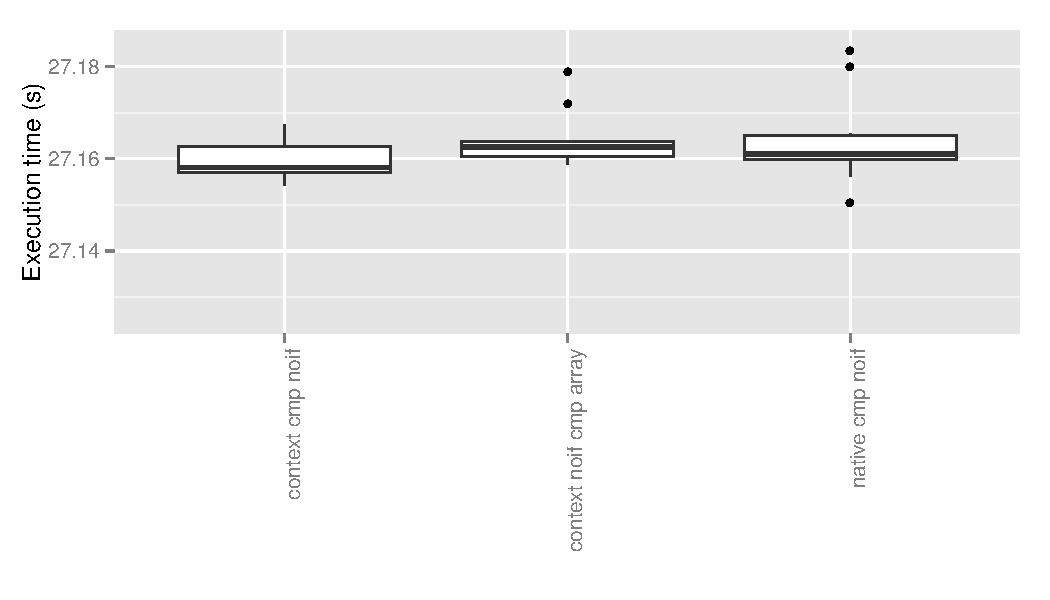
\includegraphics[scale=0.8]{benchmarkcmp}
\caption[Comparison with contextual values.]{Comparison of contextual values to native performance of variables~\cite{raab2014program}.
The figure shows a boxplot with linear scale.
Black dots are outliers, i.\,e., measurements not within $1.5*$interquartile range~\cite{raab2015global}.}
\label{fig:benchmarkcmp}
\end{figure}

Figure~\ref{fig:benchmarkcmp} shows the measurement of our implementation (``context cmp noif'', as presented in \secref{frontend-implementation-choices}) and the measurement with native non-contextual variables (``native cmp noif'').
In our benchmark, the implementation has no run-time overhead compared to native non-contextual variables~\cite{raab2014program}.

\begin{figure}[htp]
\centering
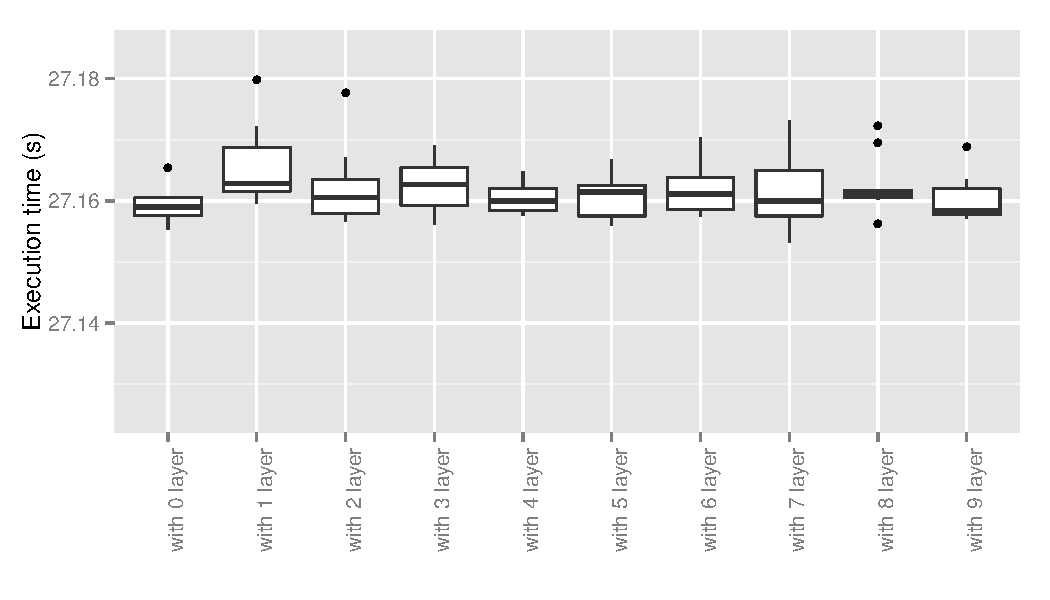
\includegraphics[scale=0.8]{benchmarkwith}
\caption[Access with active layers.]{Access with active layers~\cite{raab2014program}.}
\label{fig:benchmarkwith}
\end{figure}


As shown in Figure~\ref{fig:benchmarkwith}, increasing the number of active layers does not measurably affect the performance.
All differences are within 20 milliseconds.
Because of the huge number of loop iterations (100 billion), accessing contextual values is the dominant factor, and activating layers is negligible~\cite{raab2014program}.

\subsubsection{Discussion}

The reason for the absence of performance overhead is simple:
Compilers perform aggressive optimizations---such as inlining the method that accesses the cache of the contextual value---completely eliminating the performance overhead.
There is, however, no guarantee that the compiler actually does such optimizations.

We answer \rqref{evaluation-frontend-performance}:
\rqEvaluationFrontendPerformance*

\begin{finding}
In our model accessing contextual values can be without overhead---regardless of the number of active layers.
Only constant memory overhead occurs for each contextual value.
\end{finding}

API users do not have to restrict the use of contextual values directly in loops and performance-critical code, fulfilling the requirement:
\reqFast*
Avoiding non-context-aware copies of contextual value makes sure that context and updates are always considered, helping in the requirement:
\reqConsistency*





\rqsubsection{evaluation-frontend-multi-thread-overhead}{Web Server: Multi-thread Overhead}
\label{sec:evaluation-benchmark-web-server}

Here we benchmark the first version of the Web server introduced in \secref{implication-embedded}.
We exclusively use the multi-threaded contextual values of \elektra{}'s frontend.

\subsubsection{Method 1}
\label{sec:web-server-method}

We conducted the first benchmark on the EliteBook (see \secref{hardware}).
We measured replies per seconds by executing ^httperf^ using the arguments~\cite{raab2015global}:

\begin{code}[language=bash,numbers=none]
httperf --hog --num-conn=600000 --rate=6000 --server localhost
\end{code}

We determined ^num-conn^ and ^rate^ by optimizing for highest throughput with close-to-zero errors.
To make the setup better reproducible we did not manually tamper the device.
Instead we implemented a loop simulating a tampering event every N nanoseconds~\cite{raab2015global}:

\begin{code}[language=Cpp]
while (!shutdown)
{
	tc.activate<Tamper> ();
	std::this_thread::sleep_for (N);
	tc.deactivate<Tamper> ();
	std::this_thread::sleep_for (N);
}
\end{code}

\subsubsection{Result 1}

The loop produced a high number of layer activations and deactivations but even with only a nanosecond delay ($N=1$) we could not measure any decay of replies per seconds.
Only by removing the delay altogether we experienced slowdown~\cite{raab2015global}.

\subsubsection{Method 2: Realistic Long-held Locks}

We suspected that the slowdown is caused by internal synchronization barriers of the ^Coordinator^.
To explore this effect, we started with a realistic setup:
The source code, responsible for serializing configuration settings, needs to hold a lock.
We wrote an endless loop executed in the background to continuously require and release a lock while serializing configuration settings.

\subsubsection{Result 2}

In this scenario, again we could not measure any performance decay~\cite{raab2015global}.

\subsubsection{Method 3: Enforced Long-held Locks}

Due to lack of realistic setups, we enforced locking of the internal synchronization barriers for a fixed time of 10 milliseconds.
Then we vary the time variable $L$, during which the internal synchronization barriers are not locked~\cite{raab2015global}:


\begin{code}[language=Cpp]
while (!shutdown)
{
	std::this_thread::sleep_for (milliseconds (L));
	t.syncLayers ();
	std::unique_lock<std::mutex> l = c.requireLock ();
	std::this_thread::sleep_for (milliseconds (10));
}
\end{code}

The method ^requireLock^ returns a lock for the internal synchronization barriers.
With ^unique_lock^ we keep this lock until the end of the block implementing the loop, i.\,e., until the next loop iteration starts.
In this loop we always lock internal synchronization barriers for 10 milliseconds, while the unlocked time is controlled by $L$.


\subsubsection{Result 3}

\begin{figure}[htp]
\centering
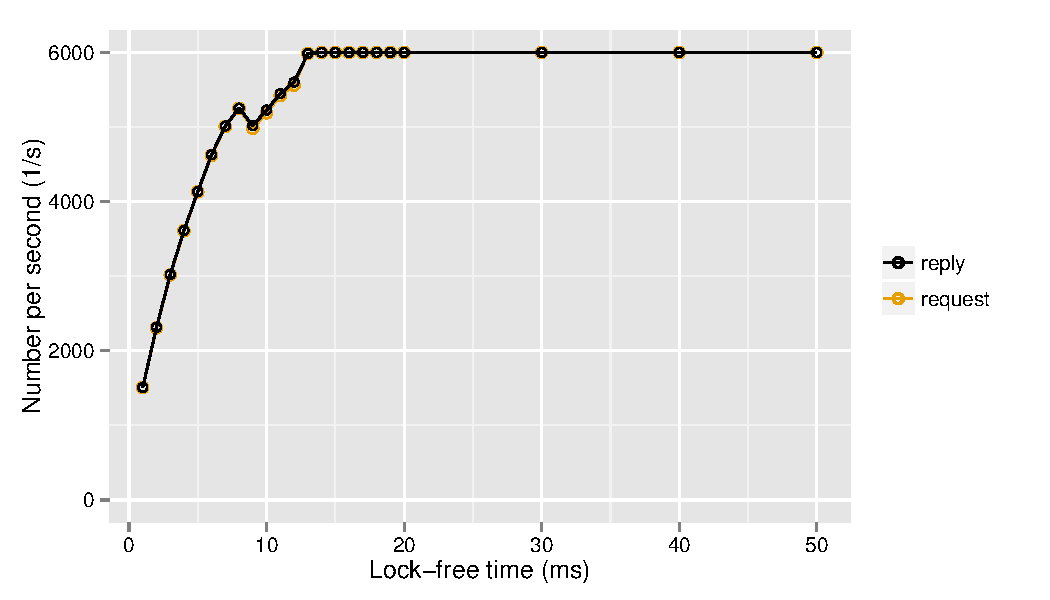
\includegraphics[width=\columnwidth]{lock}
\caption[EliteBook: HTTP requests and replies.]{HTTP replies and requests per second measured using the EliteBook.
Requests nearly perfectly overlap with the replies, and are thus hardly visible in the graph.
We increase the lock-free time $L$ in milliseconds.
The time $L=10$ corresponds to \p{50} lock-free time.
We measure both reply and requests to indicate the occurred errors~\cite{raab2015global}.}
\label{fig:lock}
\end{figure}

As we see in Figure~\ref{fig:lock}, with 14 milliseconds,
\newcommand{\unlocktime}{\p{58.3}}
i.\,e.\ \unlocktime{}
unlocked time, we achieve the full throughput time of 6000 replies per second.
With shorter lock-free periods requests and replies per seconds descent.
A difference between requests and replies is an unwanted error rate.%
{\parfillskip=0pt plus .8\textwidth \emergencystretch=.5\textwidth \par}

\subsubsection{Method 4: Embedded Single-processor System}

On a single-processor system the picture looks differently.
We again use the loop of Method 1.
In the next benchmark we started the Web server on the Raspberry Pi.
The benchmark tool ^httperf^ was running on the EliteBook.
The two devices were connected via an 100MB/s switch.
When optimizing the throughput rate with minimal error rate, we found 150 replies per second to be the maximum.
Therefore, we used the following arguments~\cite{raab2015global}:%
{\parfillskip=0pt plus .8\textwidth \emergencystretch=.5\textwidth \par}

\begin{code}[language=bash,numbers=none]
httperf --hog --num-conn=15000 --rate=150 --server pi
\end{code}

\subsubsection{Result 4}

\begin{figure}[htp]
\centering
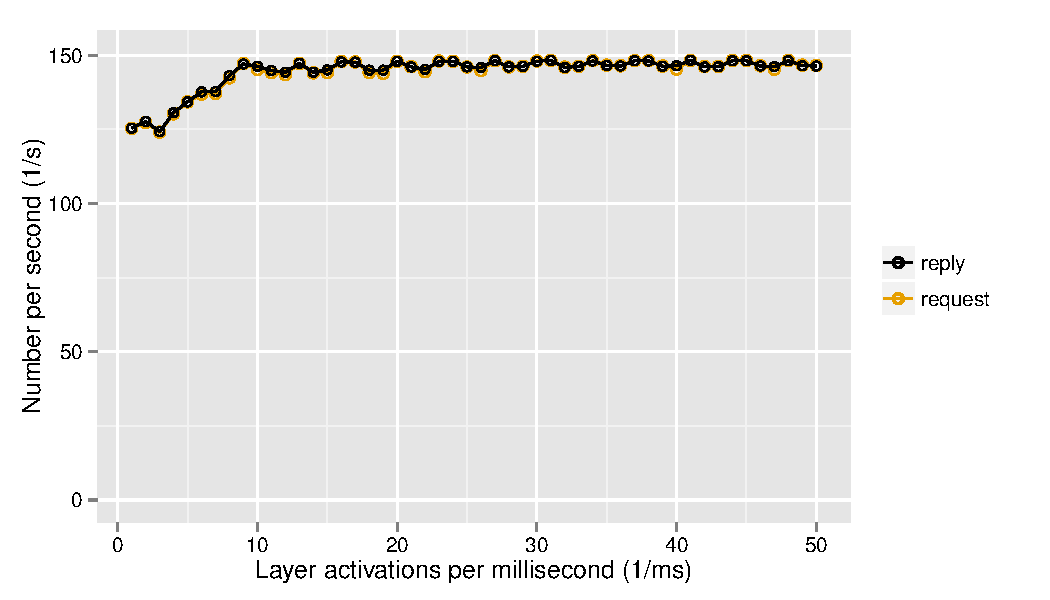
\includegraphics[width=\columnwidth]{piweb}
\caption[Raspberry Pi: HTTP requests and replies.]{HTTP requests and replies per seconds using Raspberry Pi.
We decrease layer switches per milliseconds ($N$).
We show both requests and replies to make visible that the error rate is low~\cite{raab2015global}.}
\label{fig:piweb}
\end{figure}

As we see in Figure~\ref{fig:piweb}, in this single-core embedded setup a performance decay is clearly visible.
The decay starts at a sleep time of around 7 milliseconds~\cite{raab2015global}.

\subsubsection{Discussion}

We do not expect enforced long-held locks to be a problem because it is a programmer's error to lock the ^Coordinator^ for such a long time~\cite{raab2015global}.
If we use expensive serialization techniques\footnote{In the benchmarks, we did not find a serialization technique expensive enough to create a problem. But, for example, network delays of 10 milliseconds would be equivalent to forced locks of 10 milliseconds.}, we easily avoid long locks with the following source code:

\begin{code}[language=Cpp]
KeySet duplicate;
{
	std::unique_lock<std::mutex> l = c.requireLock ();
	duplicate = deepDup (ks);
}
// serialize without holding the lock
kdb.set (duplicate);
\end{code}

Duplicating a key set is, compared to the serialization, an efficient operation.
Nevertheless, we did not come in a situation, which would require the additional two lines of code (lines 1 and 4), answering \rqref{evaluation-frontend-multi-thread-overhead}:
\rqEvaluationFrontendMultiThreadOverhead*

\begin{finding}
We found \elektra{} to be suitable for an embedded Web server setup, even with a high number of layer switches.
The current implementation of \elektra{} is sensitive to long-held locks.

We found multi-thread layer switches to be more efficient in multi-core setups.
In multi-core setups, the task of switching layers is done in another thread as background task.
\end{finding}








\rqsubsection{evaluation-frontend-performance-comparison}{Performance Comparison}

We address \rqref{evaluation-frontend-performance-comparison}:
\rqEvaluationFrontendPerformanceComparison*

\subsubsection{Method}

For the following benchmarks, we again use ^gettimeofday^ with ^Timer^.
Each benchmark invokes specific operations 100,000 times.
We reduced the number of invocations because the following operations are more expensive.
We measured overhead of ^ksLookup^ using a small key set searching for a non-present key.
The operation ^context.evaluate^ (see \defref{context-evaluate}) is used to replace 3 \empha[context placeholder]{context placeholders} in a 43 characters long string.
The operation ^switch^ means that we use ^activate^ followed by ^deactivate^.
For ^with^$N$ and ^switch^$N$ benchmarks 50,000 loop iterations are enough to perform 100,000 invocations.
We started each benchmark eleven times.
We report the results of benchmarks executed on the EliteBook~\cite{raab2015global}.

\subsubsection{Result}






\begin{figure}[htp]
\centering
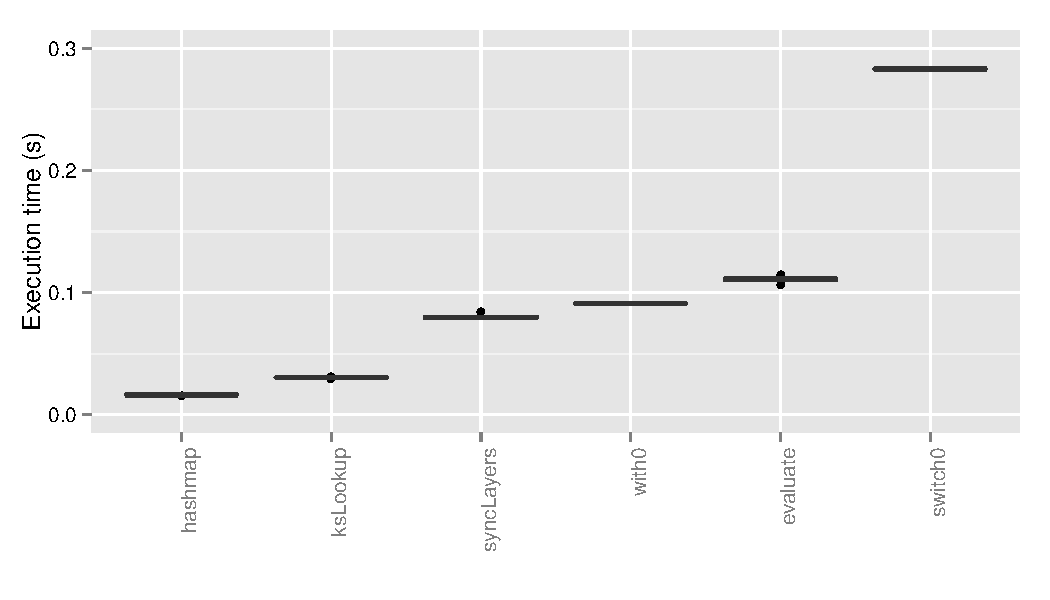
\includegraphics[width=\columnwidth]{lookup}
\caption[EliteBook: Performance of operations.]{Comparison of the duration of operations executed on the EliteBook~\cite{raab2015global}.}
\label{fig:lookup}
\end{figure}

As shown in \figref{lookup}, the C++11 hash map lookup is the fastest operation ($0.016$~seconds).
The lookup in \elektra{}'s KeySet (^ksLookup^) is about twice as slow ($0.03$~seconds).
The operation ^syncLayer^ takes about $0.08$~seconds.
The operation \linebreak \texttt{context.evaluate} (named ^evaluate^ in \figref{lookup}) needs $0.11$~seconds~\cite{raab2015global}.%
{\parfillskip=0pt \emergencystretch=.5\textwidth \par}

\begin{figure}[htp]
\centering
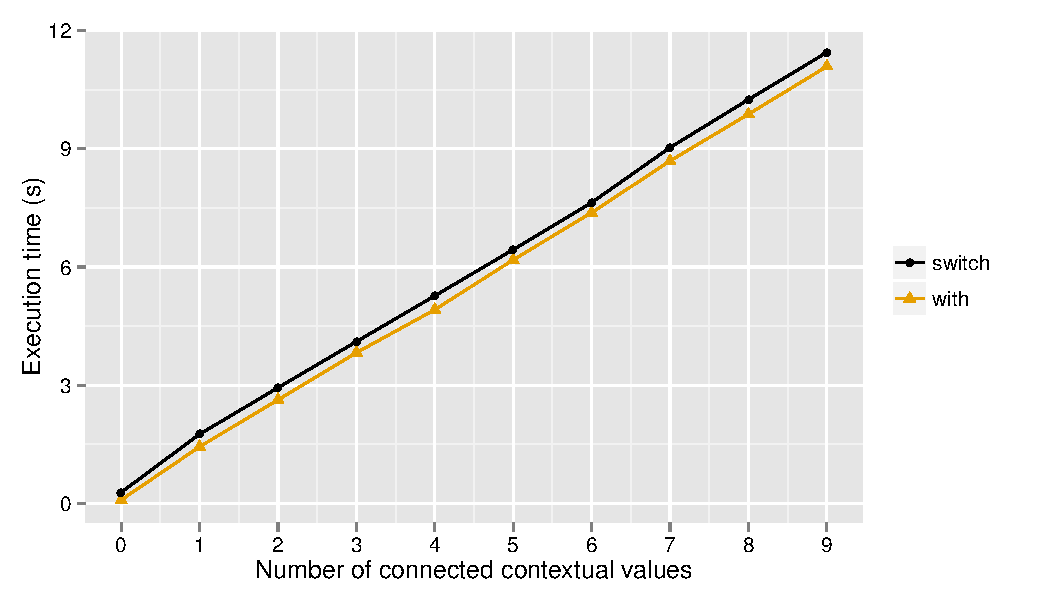
\includegraphics[width=\columnwidth]{switch}
\caption[Comparison of layer switches.]{Comparison of layer switches (i.\,e., the methods \texttt{activate} and \texttt{deactivate}) and the method \texttt{with}.
We vary the number of connected contextual values~\cite{raab2015global}.}
\label{fig:switch}
\end{figure}

As demonstrated in Figure~\ref{fig:switch}, the number of connected contextual values influences the execution time~\cite{raab2015global}.


\subsubsection{Discussion}

We expect ^ksLookup^ to be slower than a hash map lookup due to its additional features.
For example, cascading lookups have extra treatment to handle specifications and namespaces.
From \figref{switch}, we conclude that costs increase linearly in time with a larger number of connected contextual values.
The difference between ^switch^ and ^with^ is a small constant offset~\cite{raab2015global}, answering \rqref{evaluation-frontend-performance-comparison}:
\rqEvaluationFrontendPerformanceComparison*

\begin{finding}
All of \elektra{}'s operations have little overhead if only a few values are connected.
The operations ^activate^ and ^with^ have linearly more execution time depending on the number of connected contextual values.

\begin{implication}
Developers need to take care to only connect contextual values with layers as needed.
\end{implication}
\end{finding}









\rqsubsection{evaluation-frontend-resource-utilization}{Resource Utilization}
\label{sec:resource-utilization}

We deal with \rqref{evaluation-frontend-resource-utilization}:
\rqEvaluationFrontendRessourceUtilization*

\subsubsection{Method}

We measured the binary sizes of executables using the command ^ls^.

\subsubsection{Result}

The binary of the stripped library ^libelektra.so.0.8.10^, i.\,e.\ \elektra{Lib}'s core, has a size of 109,912 bytes on ^amd64^, and 98,456 bytes on ^armhf^.
The over 50 plugins range from 8 kilobytes for an iteration plugin to 100 kilobytes for a type-checker plugin.
To parse INI files, we need an additional plugin that occupies 22,760 bytes (libelektra-ini).
To resolve file names in a multi-process-safe and multi-thread-safe way, 47,560 extra bytes are needed (libelektra-resolver)~\cite{raab2015global}.
As comparison, the library ^libxml2.so.2.8.0^ (that is used by others for the same purpose, i.\,e., configuration file validation and parsing) requires 1,436,984 bytes on ^amd64^ and 1,196,108 bytes on ^armhf^.


\subsubsection{Discussion}

Because of the high degree of modularity within our implementation, users can choose which plugins to install.
This way, only space for needed functionality is occupied---leading us to the answer of \rqref{evaluation-frontend-resource-utilization}:
\rqEvaluationFrontendRessourceUtilization*

\begin{finding}
\elektra{} has a smaller binary size than XML libraries, about $\frac{1}{10}$ if including typical functionality.

\begin{implication}
\elektra{} is well suited for embedded systems and otherwise resource-constrained systems.
\end{implication}
\end{finding}




\rqsubsection{evaluation-frontend-comparison}{Activation of Contextual Values}

We want to respond to \rqref{evaluation-frontend-comparison}:
\rqEvaluationFrontendComparison*

\subsubsection{Method}


We benchmarked \elektra{} on the EliteBook as described in \secref{hardware}.
Because a long time passed during these experiments, we upgraded the operating system to Debian GNU/Linux Jessy 8.4 ^amd64^, which has the compiler GCC \mbox{4.9.2-10} as default.
We again did not alter the systems for performance improvements but on our system the maximum number of file descriptors was increased to $65,536$~\cite{raab2016persistent}.

We created four microbenchmarks.
Each of them measures the cost of activating layers 1,000 times.
Every shown number is the median value from 11 executions.
The main design criteria for the microbenchmarks are their merits for helping in deciding which activation strategy to use.
The results and discussions of all four microbenchmarks follow afterwards.
For all benchmarks, we use the following variables~\cite{raab2016persistent}:

\begin{code}[language=Cpp,escapeinside={(*@}{@*)}]
Timer t;           // see  (*@\color{purple}\secref{timer}@*)
ThreadContext c;   // see  (*@\color{purple}\secref{thread-context}@*)
Value<long> tcv;   // contextual value for benchmark
\end{code}

Our first benchmark (\strong{activate}) measures layer activations using layer classes ^Layer0^ to ^Layer8^~\cite{raab2016persistent}.
In this benchmark, we do not activate contextual values, but we pass $n$ contextual values using the parameter ^cv^.
The contextual values ^cv^ and ^tcv^ are connected with the context ^c^.
The parameter $n$ ranges from $0$ to $9$, activating no layer for $n=0$, activating ^Layer0^ for $n=1$, activating ^Layer0^ and ^Layer1^ for $n=2$, etc.

\begin{code}[language=Cpp]
void benchmarkActivate (std::vector<Value<long>> & cv, long n)
{
	t.start ();
	for (long i = 0; i < 1000; ++i)
	{
		if (n>0) c.activate<Layer0> ();
		// ..
		if (n>8) c.activate<Layer8> ();
		x ^= tcv + tcv;
	}
	t.stop ();
}
\end{code}

We take the measurement between line~3 and line~11.
Lines~6--8 contain the relevant parts to be measured.
We added line~9 to disable aggressive compiler optimizations that would eliminate the loop.
This line does not affect the measurement because it only reads contextual values.
We know this operation is as fast as reading native variables~\cite{raab2016persistent}.



In the second microbenchmark (\strong{activate cv}), we avoided context-unaware activation and used the contextual-value-activation feature introduced in \secref{mobile}.
In the lines 6--8, we activated $0$ to $9$ contextual values (the $9$ contextual values are called ^cv[0]^ to ^cv[8]^), which activated $0$ to $9$ layers~\cite{raab2016persistent}:


\begin{code}[language=Cpp]
void benchmarkActivateCV (vector<Value<long>> & cv, long n)
{
	t.start ();
	for (long i = 0; i < 1000; ++i)
	{
		if (n>0) c.activate (cv[0]);
		// .. <continues on the next page>
\end{code}

\begin{code}[language=Cpp,firstnumber=8]
		if (n>8) c.activate (cv[8]);
		x ^= tcv + tcv;
	}

	t.stop ();
}
\end{code}



In the third benchmark (\strong{sync}), we facilitate the ^sync^ feature as described in \secref{mobile}.
Line~7 synchronizes all $n$ contextual values passed as argument.
For every activation every contextual value must be recalculated.
Here we do not reload contextual values from the execution environment~\cite{raab2016persistent}:


\begin{code}[language=Cpp]
void benchmarkSync (std::vector<Value<long>> & cv)
{
	// cv.values () contains 0 to n contextual values
	t.start ();
	for (long i = 0; i < 1000; ++i)
	{
		c.sync ();
		x ^= tcv + tcv;
	}
	t.stop ();
}
\end{code}

In the forth microbenchmark (\strong{reload}), we additionally synchronized the execution environment.
In this benchmark, we parsed configuration files from hard disk before every ^sync^.
As described in~\secref{kdb-semantics}, due to an optimization repeated invocations of ^kdb.get^ would not repeatedly parse unchanged configuration files.
Therefore, we used a new ^KDB^ instance for every ^kdb.get^ (lines 3--4, and line~8)~\cite{raab2016persistent}, which forced ^kdb^ to parse the configuration file:

\begin{code}[language=Cpp]
void benchmarkReload (std::vector<Value<long>> & cv)
{
	std::vector<KDB> kdb;
	kdb.resize (1000);
	t.start ();
	for (long i = 0; i < 1000; ++i)
	{
		kdb[i].get (cv.values ());
		c.sync ();
		x ^= tcv + tcv;
	}
	t.stop ();
}
\end{code}



\subsubsection{Result}

\begin{figure}[htp]
\centering
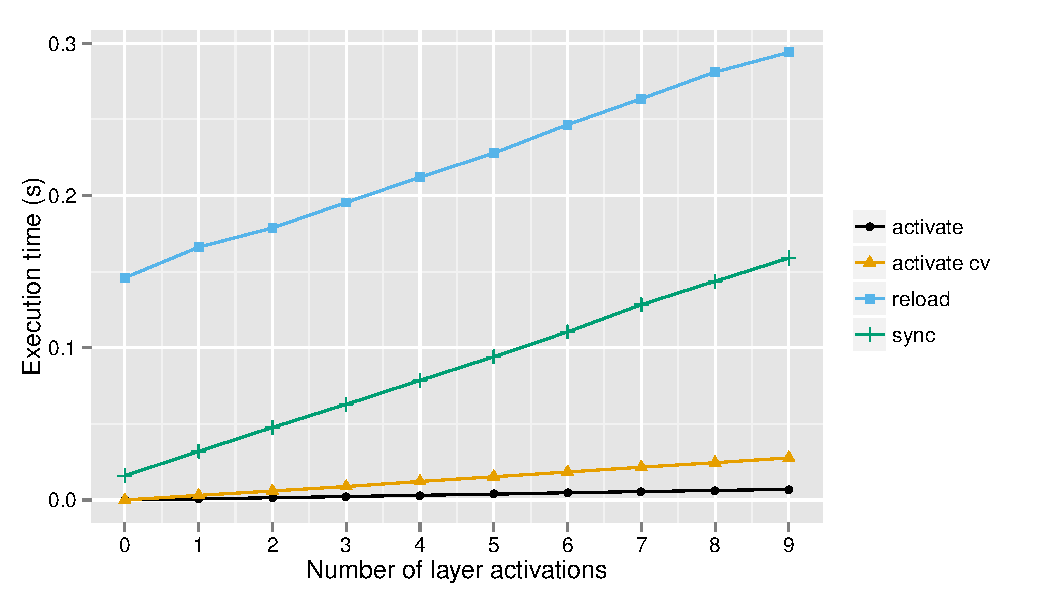
\includegraphics[width=\columnwidth]{switchmobile}
\caption[Comparison of context changes.]{Comparison of 1,000 iterations with four microbenchmarks:
\strong{activate:} directly activate layers;
\strong{activate cv:} activation of contextual values;
\strong{reload:} sync with reloading from persistent storage; and
\strong{sync:} sync all contextual values in memory.
We increase the number of activations of layers or contextual values~\cite{raab2016persistent}.}
\label{fig:switchmobile}
\end{figure}

The results of all four microbenchmarks are displayed in \figref{switchmobile}.
Again the number of activations is dependent on the contextual values to be updated.
More flexible activation strategies have additional costs (\strong{activate cv} and \strong{sync}).
Round trips to persistent, textual configuration files add a constant overhead (\strong{reload})~\cite{raab2016persistent}.

\subsubsection{Discussion}

\figref{switchmobile} indicates that we have a linear increase of execution time if more contextual values or layers are involved.
The offset in the \strong{reload} benchmark is large but constant, only measuring the time to parse the configuration file~\cite{raab2016persistent}.
We answer \rqref{evaluation-frontend-comparison}:%
{\parfillskip=0pt \emergencystretch=.5\textwidth \par}
\rqEvaluationFrontendComparison*

\begin{finding}
The run-time overhead of activating contextual values is comparable to activations of layer classes.
Higher-level abstractions such as synchronizing all layers are more expensive.
\end{finding}









\rqsubsection{evaluation-frontend-embedded-activation}{Web Server: Inter-process Layers}

Here we benchmark the second version of the Web server, which has been introduced in \secref{implication-embedded}.
We already benchmarked the first version of the Web server in \secref{evaluation-benchmark-web-server}.
Here we benchmark inter-process layers, answering \rqref{evaluation-frontend-embedded-activation}:
\rqEvaluationFrontendEmbeddedActivation*

\subsubsection{Method}

We extend the Web server benchmark to use reloading from configuration settings in the way as ^benchmarkReload^ does.
Although in our setup we use a thread for context changes, by design several processes can be used instead.
In this benchmark we found 2,200 requests per seconds as highest throughput without errors.
Again we use ^httperf^ on the EliteBook via ^localhost^~\cite{raab2016persistent}:

\begin{code}[language=bash,numbers=none]
httperf --hog --timeout=1 --rate=2200 --num-conn=50000 \
        --num-call=1 --server=localhost
\end{code}


\subsubsection{Result}

\begin{figure}[htp]
\centering
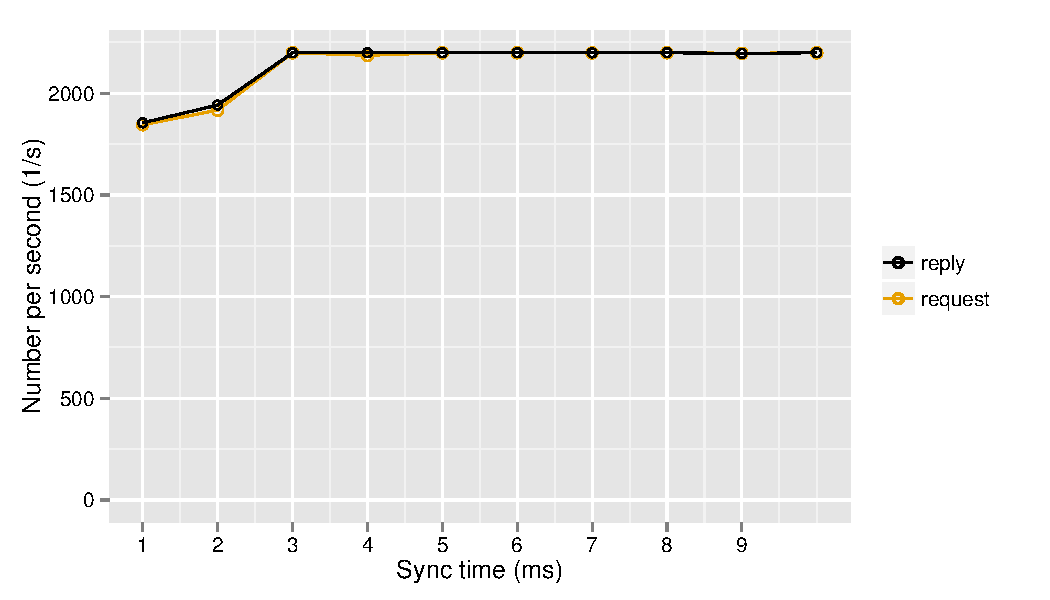
\includegraphics[width=\textwidth]{lockmobile}
\caption[Request and reply rate of a Web server.]{Request and reply rate of a Web server.
The \strong{sync time} is the wait interval given in milliseconds.
The interval is used to sleep until the next activation of inter-process layers~\cite{raab2016persistent}.%
{\parfillskip=0pt plus .8\textwidth \emergencystretch=.5\textwidth \par}}
\label{fig:lockmobile}
\end{figure}

In Figure~\ref{fig:lockmobile}  there is an effect for \strong{sync times} below 3 milliseconds.
We see a small error rate (difference between requests and replies) in the sync times of 2 and 4 milliseconds.

\subsubsection{Discussion}

We expect that with frequent synchronizations the internal barriers in ^Coordinator^ are locked too long, reducing the throughput~\cite{raab2016persistent}.
We answer \rqref{evaluation-frontend-embedded-activation}:
\rqEvaluationFrontendEmbeddedActivation*

\begin{finding}
Different from multi-thread layer switches, inter-process layer switches have measurable overhead in a Web server setup but only for switch rates every few milliseconds.

\begin{implication}
\elektra{} is efficient enough to be used in embedded applications.
The number of context changes has a small effect, even with inter-process layer switches~\cite{raab2016persistent}.
\end{implication}
\end{finding}
























\section{Comparison: Frontends Versus Backends}
\label{sec:evaluation-comparison}

For some features it is unclear if an implementation is better done in the frontend or in the backend.
In this section we investigate \rqref{comparison-frontend-backend}:
\rqComparisonFrontendBackend*

Arguments in favor of implementing features in the backends are:
\begin{itemize}
 \item that the features are immediately available consistently for all frontends,
 \item that tools with different frontends have the same behavior, and
 \item system administrators can manipulate the specification without recompilation.
\end{itemize}
The main argument for implementations in the frontend is performance:
The code generator is not restrained by a common data structure and can introspect the specification at compile-time.
Nevertheless, we recommend conducting a benchmark before features are woven into the frontends.
Unfortunately, such benchmarking is time-consuming and it is unrealistic that every decision is backed up by a benchmark.
Thus we demonstrate in a benchmark a more complicated algorithm that features several aspects relevant for such decisions.
We guide through a benchmark for cascading lookup with links and namespaces, as defined in \secref{lookup-by-spec}.
We took this algorithm because of its high number of property lookups.



\subsection{Method}

We conducted the benchmarks again on the EliteBook as described in \secref{hardware}.
The operating system at that time was Debian GNU/Linux Wheezy 7.5, with GCC compiler version \mbox{4.7.2-5}.
We ran every benchmark eleven times for the boxplots~\cite{raab2015kps}.

We implemented two variants of the cascading lookup algorithm: for the backend and for the frontend~\cite{raab2015kps}.
Here we summarize important differences:
\begin{description}
\item[In the backend variant]
properties needed for decisions are available via metadata.
We cannot know in advance which properties are present.
Instead in this variant, we always need to exhaustively introspect every relevant property.

As precondition, applications need to be able to successfully read the configuration specification.
To avoid this precondition to fail, we recommend having a built-in copy of the specification.
Then the application starts up without a working key database as demonstrated in \secref{approach-guarantees}~\cite{raab2015kps}.

\item[In the frontend variant]
the source code implementing the properties is woven into the application's source code.
In this variant, the code generator only adds source code for specified properties.
If no link is specified, we get the same source code as if the feature did not exist at all.
This variant avoids any overhead if no properties are present.
\end{description}

We implemented and measured both the frontend and the backend variant.
We measure ^ksLookup^ with $N$ \property{override} links.
We make 200,000 lookups with a contextual value.
To make sure that we call ^ksLookup^, we synchronize the contextual value's cache for every access.
We always use a ^KeySet^ with five keys.
The key to look up has $N=0$ to $9$ \property{override} properties~\cite{raab2015kps}.

\begin{example}
The key with 2 properties \property{override} is~\cite{raab2015kps}:

\begin{code}[morekeywords={override,long},escapeinside={(*@}{@*)}]
[benchmark/#2]
  default:=33
  type:=unsigned_long
  override/#0:=/benchmark/(*@override@*)/#0
  override/#1:=/benchmark/(*@override@*)/#1
\end{code}
\end{example}

As next step, we benchmark a word counting tool that reimplements the standard UNIX tool ^wc^.
We intensively used the property ^override^ (algorithm given in \secref{lookup-by-spec}) in \elektra{Spec} for the elektrified tool ^wc^.
We utilized the technique as described in \exref{override-argument} to implement the check if different features are combined~\cite{raab2015kps}:


\begin{code}[morekeywords={long,override}]
[sw/wc/show/max_line_length]
  type:=boolean
  default:=false
  opt:=L
  opt/long:=max_line_length
[sw/wc/show/no_default_args]
  type:=boolean
  default:=false
  override/#0:=/sw/wc/show/lines
  override/#1:=/sw/wc/show/words
  override/#2:=/sw/wc/show/chars
  override/#3:=/sw/wc/show/bytes
  override/#4:=/sw/wc/show/max_line_length
\end{code}

As input of the ^wc^ tool, we used a \LaTeX~file of 32 kilobyte size.
We facilitated Callgrind 3.7.0 to profile the whole application~\cite{raab2015kps}.



\subsection{Result}

\begin{figure}[htp]
\centering
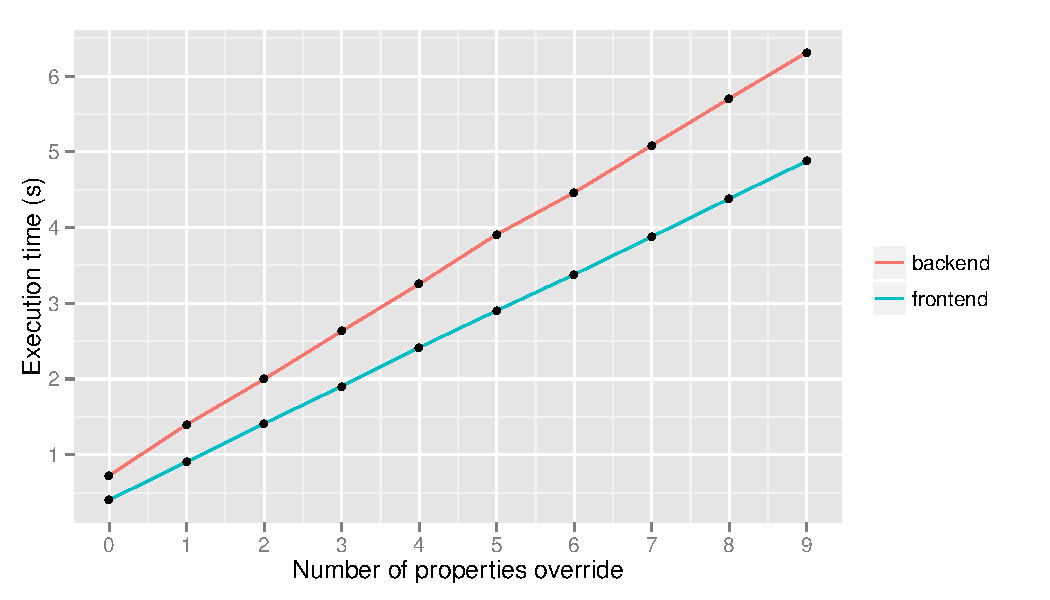
\includegraphics[width=\textwidth]{mean2}
\caption[Lookup time in backend and frontend implementation variant.]{Lookup time in backend and frontend implementation variant.
We use a linear scale~\cite{raab2015kps}.}
\label{fig:combined}
\end{figure}

\figref{combined} shows the growth in execution time depending on the number of \property{override} properties.
In the figure already for 0 properties \property{override}, the overhead for the backend is $1.8$ times higher, and then it grows \p{22} faster~\cite{raab2015kps}.

\begin{figure}[htp]
\centering
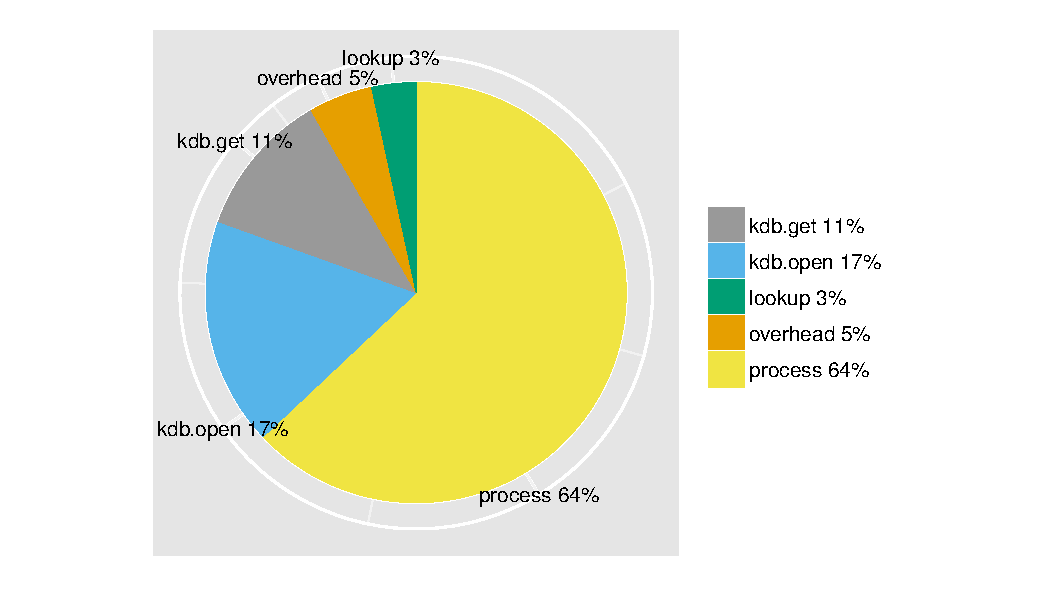
\includegraphics[width=\textwidth]{wc}
\caption{Overhead of an \empha[elektrify]{elektrified} application~\cite{raab2015kps}.}
\label{fig:wc}
\end{figure}

For \figref{wc}, we grouped the counted instructions of the ^wc^ application into~\cite{raab2015kps}:
\begin{description}
\item[process:] the main functionality of the application.
The processing of the characters in the \LaTeX~file dominates with \p{64} of the counted instructions.
\item[kdb.open:] the bootstrapping as explained in~\secref{bootstrapping}.
It takes about \p{17}, mainly due to configuration file parsing.
The configuration file parser in use is about 12 times slower than the word counter.
\item[kdb.get:] the parsing of the application's configuration file.
It costs about \p{11} of overall cycles, also mainly due to configuration file parsing.
\item[lookup:] the base costs of the lookup without property \property{override}.
\item[overhead:] the additional costs of the lookup if links are present in the specification.
Without any links, only 9 instead of 27 cascading lookups are needed.
In total, the overhead due to links of the application is \p{5} in this application.
\end{description}



\subsection{Discussion}

In microbenchmarks resolving links the frontend variant is clearly faster.
In whole applications, however, the difference is minimal.
The overhead might be caused by other factors, such as the parsing time of the additional configuration specification, and not only by the lookup itself.
We answer \rqref{comparison-frontend-backend}:
\rqComparisonFrontendBackend*

\begin{finding}
\fixtheorem
\begin{enumerate}
\item
For the benchmark we needed to turn off frontend caches to measure differences.
Without caches, the overhead for the backend is $1.8$ times higher and grows \p{22} faster~\cite{raab2015kps}.
\item
Even in an application that excessively uses links, the overhead of having the link properties present, is only \p{5}.
\end{enumerate}

\begin{implication}
Differences in overhead are little, at least for the ^ksLookup^ algorithm.
Thus features, such as links, shall be implemented in the backend.
\end{implication}
\end{finding}


























\section{Overhead of Modular Abstractions}
\label{sec:evaluation-modular}

It is well-known that modular abstractions usually come with a price tag: overhead.
In this section we benchmark the vertical and horizontal modular abstraction as introduced in \secref{modular-abstractions}, answering \rqref{overhead-modularity}:
\rqOverheadModularity*

\subsection{Method}

We benchmarked \elektra{Spec} on the EliteBook as described on \secref{hardware} with the operating system Debian GNU/Linux Wheezy 8.2 ^amd64^.
We employed the compiler GCC \mbox{4.9.2} with the compiler option ^-O2^~\cite{raab2016improving}.
The benchmark setups are described in the individual sub-sections.


\subsection{Vertical Modularity}

\subsubsection{Method}

To evaluate the overhead of vertical modularity, we increase the number of present mountpoints for an application.
With zero mountpoints, \elektra{} serializes the key set into the \empha{default mountpoint}.
For more mountpoints, we use the property \property{mountpoint}.%
{\parfillskip=0pt \emergencystretch=.5\textwidth \par}
\begin{example}
With three mountpoints, we have the following specification~\cite{raab2016improving}:

\begin{code}
[benchmark/0]
  mountpoint:=/tmp/file0
[benchmark/1]
  mountpoint:=/tmp/file1
[benchmark/2]
  mountpoint:=/tmp/file2
\end{code}
\end{example}

\subsubsection{Result}

\begin{figure}[htp]
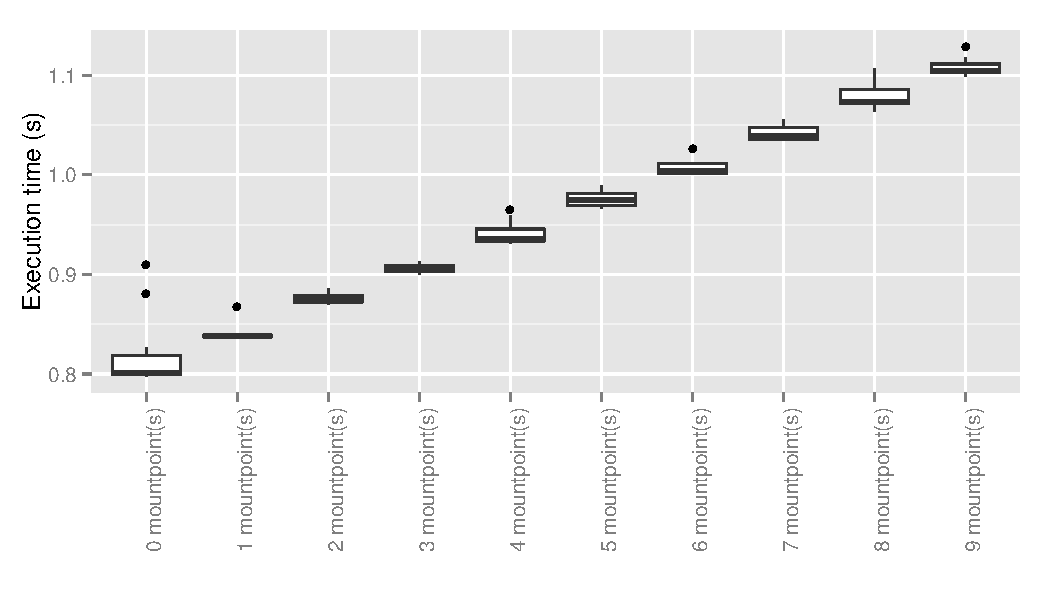
\includegraphics[width=\textwidth]{benchmark}
\caption[Access Time with increasing number of mountpoints.]{Access time using 1,000 keys with 100,000 iterations.
On the $x$-axis we increase the number of mountpoints~\cite{raab2016improving}.}
\label{fig:benchmark-access}
\end{figure}

\figref{benchmark-access} shows that the execution time for nine mountpoints is about \p{28} higher compared to the execution time with zero mountpoints.


\subsection{Horizontal Modularity}

\subsubsection{Method}

To measure the overhead of horizontal modularity, we implemented a plugin called ^iterate^.
It searches all keys for the property \property{iterate}.
The plugin \plugin{iterate} simulates an action required by most plugins in \elektra{}:
It investigates which action is required by which key.
In the benchmark, we increase the number of plugins present in one mountpoint.
Then we use ^gettimeofday^ to measure how long it takes to parse and serialize the configuration files, with the plugins present.

\begin{example}
In the benchmark with three plugins, we have the following configuration specification~\cite{raab2016improving}:\footnote{The array index at the end of the plugin name enables multiple instantiations of the same plugin.}

\begin{code}[morekeywords={needs}]
[benchmark]
  mountpoint:=/tmp/file
  infos/needs:=iterate#0 iterate#1 iterate#2
\end{code}
\end{example}


\subsubsection{Result}

We were not able to measure any overhead by adding more plugins.
When increasing the number of keys, we only increased the parsing time.
The time spent in the plugin \plugin{iterate} was too little using our measurement method~\cite{raab2016improving}.

\subsection{Discussion}

From \figref{benchmark-access} we conclude the answer to \rqref{overhead-modularity}:
\rqOverheadModularity*

\begin{finding}
\fixtheorem
\begin{enumerate}
\item
Vertical modularity, i.\,e., applications accessing the configuration files of each other, has run-time overhead correlating linearly with the number of used mountpoints.
\item
The run-time overhead of horizontal modularity, i.\,e., plugins executed during configuration access, is negligible.
\end{enumerate}

\begin{implication}
The overhead of \elektra{Spec} does not give reasons to avoid modularity.
Concerning performance, every feature shall be implemented as separate plugin and every application shall use its own configuration file~\cite{raab2016improving}.
\end{implication}
\end{finding}






















\section{Context Awareness without Source-code Modification}
\label{sec:evaluation-unmodified}

We practically apply our tool in large real-world applications and a systematic software-engineering process described in \secref{cose-process} to answer \rqref{unmodified}:
\rqUnmodified*



To answer the overall question, in each of the sub-sections, we respond to one of the sub-questions:
\rqUnmodifiedWhich*
\rqUnmodifiedPractical*
\rqUnmodifiedOverhead*
\rqUnmodifiedPerformance*









\subsection{Method}

For this evaluation, we chose the same 16 popular systems in the same versions as selected in \tabref{versions}.
We investigated all of these applications but here we mainly report on browsers.
Reports of other applications are described in earlier work~\cite{raab2016unanticipated,raab2017introducing}, with similar results.

We used Debian GNU/Linux Jessie 8.1 for our evaluation.
To enable the interception of \elektra{} globally, we used ^/etc/ld.so.preload^.
This way, \elektra{}'s ^getenv^ is preferred to the system's ^getenv^ implementation.
The benchmarks were executed on the EliteBook, as described in~\secref{hardware}.
Overhead is measured using Valgrind by executing applications with and without \elektra{}~\cite{raab2016unanticipated}.
Individual methods are described in the respective sub-sections.



\subsubsection{Threats to Validity}

To mitigate measurement problems we cross-checked with two profiling tools:
We used Valgrind Callgrind and Linux Perf.

The benchmarks are conducted comparatively with the system's ^libc^.
We compared with ^getenv^ of the Eglibc 2.19 implementation.
Results may vary with other ^libc^ implementations~\cite{raab2017introducing}.

The benchmarks yield different results depending on the used configuration file formats and even depending on the size of the used configuration files.
To mitigate this problem, we took special care that our setup is realistic.
We mounted 8 different configuration files and especially chose slow storage plugins.
It should be straightforward to repeat our benchmarks measuring even less overhead than reported by us~\cite{raab2016unanticipated}.

Many alternative configuration access APIs exist, but none of them is standardized and ubiquitous.
We are positive that the results are not specific to ^getenv^ but can be reproduced for other configuration access APIs as well.
Other configuration access APIs have the same purpose and only differ in how to use them~\cite{raab2016unanticipated}.

We added logging to count the number of ^getenv^ occurrences.
Extensive logging can influence a system adversely.
To mitigate this problem, we reran all tests with deactivated logging~\cite{raab2016unanticipated}.%
{\parfillskip=0pt plus .7\textwidth \emergencystretch=.5\textwidth \par}

We did not consider applications that already were implemented with context awareness in mind.
Thus we need to exclude such applications from our claims and cannot draw general conclusions for context-aware applications.
Nevertheless, our study unveils important insights about context-aware configuration, particularly for FLOSS~\cite{raab2016unanticipated}.



\rqsubsection{unmodified-which}{Unanticipated Context Awareness}

In \secref{context-awareness}, we already demonstrated that the use of ^getenv^ is pervasive, even after startup.
Here we validate how many ^getenv^ invocations are intercepted and controlled at run-time by \elektra{}.
We show that changes in the context---and hence in the variables returned by ^getenv^---have an influence on the behavior of the application~\cite{raab2016unanticipated}, answering \rqref{unmodified-which}:
\rqUnmodifiedWhich*

\subsubsection{Method}

First we launched the applications, used the menus, and clicked on buttons of the user interface.
While doing so, we traced every ^getenv^ invocation with its parameters.
To check if ^getenv^ invocations are context aware, we changed the return values of ^getenv^ while the application was still executing.
After repeating the user-interaction, we checked for visual differences to know if the ^getenv^ invocation influenced behavior~\cite{raab2017introducing}.

The run-time analysis considers calls to ^getenv^ throughout the stack by all participating libraries, complementing our earlier source code analysis in \secref{context-awareness}.
We aim to find how often changed return values of ^getenv^ invocations in the whole stack actually modify the behavior of 5 different browsers~\cite{raab2017introducing}.

For some of the settings ($\geq$ in \tabref{unmodified-context-aware}), we lacked the resources to investigate them in detail, even though further settings are likely context aware.
The effort to determine context awareness of a single setting sometimes is immense.
For example, some configuration settings need installations of servers which use out-dated certificates.
Others require buying CPUs implementing different accelerations for cryptographic algorithms.


\subsubsection{Result}

\begin{table}[htp]
\noindent
\begin{tabularx}{\columnwidth}{ l  R  R  R  R  R }
\toprule
\multicolumn{1}{l}{\bfseries Application} &
\multicolumn{1}{R}{\bfseries \blap{\texttt{getenv} \\ all}} &
\multicolumn{1}{R}{\bfseries \blap{all \\ uniq}} &
\multicolumn{1}{R}{\bfseries \blap{later \\ uniq}} &
\multicolumn{1}{R}{\bfseries \blap{later \\ config}} &
\multicolumn{1}{R}{\bfseries \blap{context \\  aware}}
\\
\hline
Chromium   & 2,723  & 1,056    & 73 &$\geq24$& $\geq1$  \\
Curl       & 87     & 14       & 9  &       6&       6  \\
Firefox    & 8,185  & 273      & 210&     118&$\geq15$  \\
Lynx       & 1,428  & 45       & 23 &      19&      16  \\
Wget       & 13     & 7        & 1  &       1&       1  \\
\bottomrule
\end{tabularx}
\caption{Achieved context awareness in software without source code modifications~\cite{raab2017introducing}.}
\label{tab:unmodified-context-aware}
\end{table}

\tabref{unmodified-context-aware} has the following columns:
In the first column \strong{\texttt{getenv} all}, we show how often the browsers called ^getenv^ (in total).
The next column \strong{all uniq} considers the number of ^getenv^ invocations with unique parameters.
The column \strong{later uniq} exclusively displays ^getenv^ invocations with unique parameters and only after startup.
The next column \strong{later config} shows good candidates for context awareness:
They are not related to debugging, testing, and similar.
The last column \strong{context aware} presents candidates that are able to successfully modify behavior at run-time without reloading~\cite{raab2017introducing}.%
{\parfillskip=0pt \emergencystretch=.5\textwidth \par}

\tabref{unmodified-context-aware} presents the number of ^getenv^ invocations from applications started on a freshly installed Debian GNU/Linux system.
The number of invocations varies not only between applications but it depends heavily on the system it runs on, for example, the installed software.
On other machines, we detected several times more unique ^getenv^ invocations for Firefox~\cite{raab2017introducing}.
The upper bound is not necessarily the number of ^getenv^ invocations found in the source code analysis because libraries call ^getenv^, too.%
{\parfillskip=0pt \emergencystretch=.5\textwidth \par}

To give an example, let us walk through the behavior of all browsers for the environment variable ^http_proxy^.
Lynx requests ^http_proxy^ via ^getenv^ before trying to fetch content.
We can return proxies suitable for the network to seamlessly display every page without proxy errors.
Wget also requests ^http_proxy^ for every recursive download.
Curl adds even more fine-grained control: 7 additional environment variables allow us to distinguish protocols.
Firefox rereads ^http_proxy^ for every page, except when they are already in cache.
Chromium is the only browser that does not query ^http_proxy^~\cite{raab2016unanticipated}.
Instead it rereads many other environment variables such as ^GOOGLE_API_KEY^ after start-up.
In Chromium, we only found ^PRINTER_LIST^ to be exploitable for flawless context awareness.%
{\parfillskip=0pt plus .7\textwidth \emergencystretch=.5\textwidth \par}


In rare situations, context awareness leads to wrong behavior.
In these situations, developers required ^getenv^ invocations to keep returning the same values.
For example, the environment variable ^CC^ determines which C compiler is used.
With \elektra{}, the environment variable ^CC^ can be changed during the compilation of software~\cite{raab2016improving}.
Because not all compilers and linkers are completely compatible, unexpected switching in the middle of the process can lead to compilation and linker errors.


\subsubsection{Discussion}

We answer \rqref{unmodified-which}:
\rqUnmodifiedWhich*

\begin{finding}
\fixtheorem
\begin{enumerate}
\item In each of the 16 applications, user interactions caused ^getenv^ invocations.
They were often useful to influence behavior at run-time.
For Lynx even \p{42} of the ^getenv^ invocations improve context awareness.
Thus the interception is suitable to improve context awareness without changes in the source code.
\item In 4 out of 5 browsers, \elektra{} enables seamless context-aware proxy settings with ^getenv^~\cite{raab2017introducing}.


\item
Limitations include that some ^getenv^ invocations do not allow us to produce visible impact.
Context changes can lead to incorrect behavior in rare cases~\cite{raab2016unanticipated}.
\end{enumerate}

\begin{implication}
\elektra{} increases the context awareness for our evaluated applications.
Specific configuration settings were even flawlessly adapted to the context.
\end{implication}
\end{finding}


















\rqsubsection{unmodified-practical}{Case Study}

Here we show that intercepting applications without source code modifications is not only feasible but practical, answering the research question:
\rqUnmodifiedPractical*

\subsubsection{Method}

First, we conducted the entire context-oriented software engineering process as described in \secref{cose-process}.
As software without source code modifications we chose Firefox.
When changing workplaces, Firefox shall always pick~\cite{raab2017introducing}
\begin{enumerate}
\item the correct proxy, and
\item a nearby printer.
\end{enumerate}

Second, we looked at the ^open^ interception using Firefox, investigating if all configuration settings can be made context aware.

For both steps we measured the time.

\subsubsection{Result}

Within a day we conducted the process that Firefox fully-automatically selected nearby printers and proxies.
Updates in the user interface happened immediately on network changes, for example, available printers are even modified while the printer dialog is open.

We utilized one-line hooks in the ^/etc/NetworkManager^ scripts to implement the context sensor~\cite{raab2017introducing}.
Then we specified ^http_proxy^ and ^PRINTER_LIST^ as environment variables of interest (as already depicted in \secref{cose-process}) with configuration settings like:

\begin{code}[language=CfgElektra]
http_proxy/wlan/home=proxy.example.org
printer/wlan/home=laserprinter
\end{code}

\elektra{} allows us to intercept ^open^ to return handles to dynamically serialized configuration files.
To enable Firefox to reparse its configuration files, we needed 9 hours to understand the complex, historically grown AutoConfig.
Afterwards, we enabled AutoConfig with small changes exclusively in configuration files.
Future users only need to run a script to do the complete setup.
The setup does not involve source code changes but only changes Firefox's configuration settings.

In 2 more hours, we implemented a storage plugin for Firefox's configuration files.
\citet{jin2014configurations} found 1,957 configuration settings to be available in Firefox.
With ^open^ interception, we have a mechanism to make all of them context aware.


\subsubsection{Discussion}

Our approach is by no means limited to Firefox.
Instead it permits any configuration setting from any application to be adapted to context as long:
\begin{itemize}
\item \elektra{} has a binding for the respective configuration access API or has support for the respective configuration file format (for ^open^ interception).
\item The application reiterates configuration access or has support to reload its configuration settings.
\end{itemize}

Applications always repeat all relevant configuration accesses during initialization.
It is implied that every configuration access is context aware by restarting the application.
Thus when invoking external applications, all configuration accesses are by design always fully context aware.

Different interception techniques sometimes complete each other:
While ^open^ provides more settings, the printer integration in Firefox is smoother via ^getenv^ interception.%
{\parfillskip=0pt \emergencystretch=.5\textwidth \par}

\elektra{} supports any context, not only mobile workplaces.
Other examples include: user-specific privacy, security, and performance (for example, turning on hardware support).
Furthermore, context can be derived from user data such as calendars, contacts, and activities.
We did not need to validate the research questions for individual contexts:
Every context sensor collaborates with every application as implied by our complete separation of context sensors and applications.


We addressed the research question:
\rqUnmodifiedPractical*

\begin{finding}
It is practical to utilize Firefox without source code modifications along with \elektra{} in a case study.
For retrofitting context awareness in the context of flexible workplaces, we required only three actions completed within a day:

\begin{enumerate}
\item we specified contextual values,
\item we created configuration settings for each workplace, and
\item we implemented context sensors to switch layers.
\end{enumerate}

In case of Firefox, run-time serialization of configuration files is more powerful than ^getenv^ interception although the combination of both is even more capable.

\begin{implication}
\elektra{} can be practically applied to large-scale, real-world software for non-trivial use cases.
\end{implication}
\end{finding}














\rqsubsection{unmodified-overhead}{Overhead}

In this experiment we want to investigate the overhead of context changes using \elektra{} by answering \rqref{unmodified-overhead}:
\rqUnmodifiedOverhead*

\subsubsection{Method}

We activated \elektra{}'s interception technique throughout the whole experiment.
To measure the overhead of context changes, we change the key database during program execution.
This causes \elektra{} to reparse its configuration file~\cite{raab2016unanticipated}.

The setup is as follows:
We locally installed the Web server Lighttpd reachable as ^localhost^.
We used Curl to download ten files from this Web server: ^curl -o^ \allowbreak ^"#1 http://localhost/test/[1-10]"^.
The files have sizes of 1 megabyte to 10 megabytes, respectively~\cite{raab2016unanticipated}.
The file sizes were chosen to be substantially larger than any involved configuration file.
Otherwise, the overhead caused by parsing of the configuration files dominates.

We needed to take care that our experiment did not influence the control flow of the application.
For example, if we modify the ^no_proxy^ variable, searching for proxy is skipped and the performance improves unwantedly.
Thus instead, we changed ^COLUMNS^, which is requested during every download but is unrelated to the download itself~\cite{raab2016unanticipated}.%
{\parfillskip=0pt plus .8\textwidth \emergencystretch=.5\textwidth \par}


We ran three experiments and let Valgrind count the instructions for each experiment~\cite{raab2016unanticipated}:
\begin{enumerate}
\item The downloading of the ten files with \elektra{}'s interception active.
\item The downloading of the ten files with \elektra{}'s polling of changes in the configuration files (see \secref{context-changes} for different techniques of how to handle context changes).
In this case, \elektra{} tries to detect changes in the key database, although they do not happen in the second experiment.
\item The downloading of the ten files with an actual change in the key database.
Here we modified the key ^COLUMNS^ in the key database in the middle of the downloads.
This causes \elektra{} to reparse configuration files and return a new value for the next ^getenv("COLUMNS")^.
\end{enumerate}



\subsubsection{Result}

The results of the three experiments is as follows~\cite{raab2016unanticipated}:
\begin{enumerate}
\item
Without any polling or reloading of the key database, Curl needed 83,786,947 instructions.
\item
With polling of configuration files in a rate of not more than every millisecond, the configuration was retrieved 91 times instead of 4 times.
This caused Valgrind to count 91,569,790 instructions, i.\,e., an overhead of \p{9.3}.
\item
When changing ^COLUMNS^ in the middle of the downloads, Curl executed 95,248,722 instructions.
This is again an overhead of $\sim\p{4}$~\cite{raab2016unanticipated}.
\end{enumerate}

\subsubsection{Discussion}


We described a small part of all experiments measuring performance and overhead~\cite{raab2016unanticipated,raab2017introducing}.
The experiment above confirms those other experiments.
For example, we fully recompiled the source code of \elektra{} while interception was activated.
Although the compilation spawned 6847 processes\footnote{Each of which parsed configuration settings and specifications.} only \p{14} overhead occurred~\cite{raab2016unanticipated}.

We answer the question:
\rqUnmodifiedOverhead*

\begin{finding}
\fixtheorem
\begin{enumerate}
\item
In applications that work with files smaller than the involved configuration files, overhead dominates.
In intense but realistic scenarios, \elektra{} adds run-time overhead up to \p{14}~\cite{raab2016unanticipated}.

\item
Interception with polling of configuration files adds about \p{10} overhead.

\item
With changes in the key database the run-time overhead increases again by $\sim\p{4}$ in a realistic HTTP-proxy transition.
\end{enumerate}
\end{finding}

















\rqsubsection{unmodified-performance}{Performance: Layer Switches}

In this section we answer \rqref{unmodified-performance}:
\rqUnmodifiedPerformance*


\subsubsection{Method}

To evaluate the performance, we benchmarked different browsers during a proxy transition on the EliteBook as already introduced in \secref{hardware}~\cite{raab2017introducing}.
We measured the number of simulated CPU instructions with Valgrind's tool Callgrind and cross-checked with Linux Perf.
We summarize the inclusive costs, i.\,e., costs of the ^getenv^ invocation including every callee.
Because Valgrind simulates a CPU, we get deterministic results~\cite{raab2017introducing}.%
{\parfillskip=0pt \emergencystretch=.5\textwidth \par}

We conducted three experiments with Lynx and one experiment with Firefox.
We profiled Lynx because it is implemented leanly and thus has negligible startup-times.
Such a minimalist implementation enables more precise exploration of the ramifications the context changes have~\cite{raab2017introducing}.
\begin{enumerate}
\item 
First we launched Lynx without \elektra{} and visited two links by typing them in the address bar.
\item
Then we turned on \elektra{} interception and directly modified the proxy before opening the second link.
\item
In the next experiment, again with \elektra{}, we first opened a Web page, then changed the context via layers, and finally opened another Web page.
We used a contextual value with two layers: ^network^ and ^interface^.
\item
The comparison with Firefox turned out to be more difficult because it consumes resources even without any user interaction.
The startup-times of Firefox using Valgrind are nearly two minutes, which made it implausible to measure the relevant time precisely enough.
Therefore, we could not do a comparative analysis by the total count of instructions with and without \elektra{}.
Instead we estimated the overhead by analyzing the profile data.
\end{enumerate}


\subsubsection{Result}


The results of the four benchmarks are~\cite{raab2017introducing}:
\begin{enumerate}
\item
Without context-aware interception, Valgrind counted 92,888,073 instructions (median of three Valgrind invocations).
The ^getenv^ invocations used \p{0.33} of these instructions.
\item
If we modified ^env/override/http_proxy^ directly (not changing layers as it normally should be done), we counted 114,049,336 instructions (this is about \p{18.5} more instructions than from Benchmark~1) of which ^getenv^ uses \p{24.51}.
\item
If we changed a layer value before opening a second link, the ^getenv^ invocations used \p{25.27} of all instructions.
\item
Firefox required 20,362,848,539 instructions to start up and to display two Web pages.
Summing up all costs from the \elektra{} library results in 68,750,481, i.\,e., \p{0.39} (maximum value of two measurements). % 32,351,030 instructions (i.\,e., \p{0.16}).
The function ^g_getenv^ (a wrapper of ^getenv^ in Firefox) needed 16,614,089 instructions (i.\,e., \p{0.08}) rather than 22,703 instructions (i.\,e., \p{0.00}) without \elektra{}.
\end{enumerate}


\subsubsection{Discussion}

We respond to \rqref{unmodified-performance}:
\rqUnmodifiedPerformance*

\begin{finding}
In minimalist applications, such as Lynx, \elektra{} caused \p{18.5} to \p{25.27} overhead.
For feature-rich applications the overhead was below \p{1}.

The performance difference between directly modifying the configuration values and changing layer values is minimal:
It is less than one percentage point more overhead in ^getenv^'s instructions.
\begin{implication}
Developers shall prefer to facilitate contextual values and shall change configuration values indirectly via layers.
\end{implication}
\end{finding}






\subsection{Discussion}

We answer \rqref{unmodified} about intercepting applications without source code modifications:
\rqUnmodified*

\begin{finding}
It is practical and feasible to intercept configuration access API invocations from applications without source code modifications.

Even for large-scale legacy applications, where rewriting the application for more context awareness would be an immense effort, adding context awareness with \elektra{} has little time effort (hours to days) and overhead ($\sim\p{1}$ for feature-rich applications).
\end{finding}
